\newpage
\section{Limiti}
\subsection{Intorni}
\begin{definition}[Intorno]
    Dato $x_0 \in \mathbb{R}$ si dice \textbf{intorno} di $x_0$ un insieme del tipo $(x_0 - \epsilon, x_0 + \epsilon)$ dove $\epsilon \in \mathbb{R}$, e $\epsilon > 0$. Inoltre $\epsilon$ si dice raggio dell'intorno
\end{definition}
\begin{itemize}
    \item Un insieme del tipo $[x_0, x_0 + \epsilon]$ si dice \textbf{intorno destro} di $x_0$.
    \item Un insieme del tipo $[x_0 - \epsilon, x_0]$ si dice \textbf{intorno sinistro} di $x_0$.
\end{itemize}
\begin{definition}
    Se $x_0 = +\infty$ un intorno di $x_0$ è un insieme del tipo $(a, +\infty)$\footnote{$(a, +\infty)$ è una semiretta} dove $a \in \mathbb{R}$
\end{definition}
\begin{definition}[Punto di accumulazione]
    Dato $A \subset \mathbb{R}$ e $x_0 \in \overline{R}$ $x_0$ si dice \textbf{punto di accumulazione} per A se $\forall \: U$ intorno di $x_0$ risulta che $U \cap A \setminus \{x_0\} \neq 0$
\end{definition}
Questa definizione vuol dice che "vicino" a $x_0$ ci sono altri punti di A oltre a $x_0$ ($x_0$ potrebbe anche non appartenere ad A).
\begin{example}
    Prendiamo un intervallo A = (2, 3).
\end{example}
Se prendiamo un punto $x_0$ che appartiene a A, quindi $x_0 \in (a,b)$, allora ogni intorno di $x_0$ interseca A in infiniti punti, quindi $x_0$ è un punto di accumulazione di A.\\
\begin{definition}[Intorno bucato]
    Se invece non andiamo a considerare $x_0$ nel suo intorno si dice \textbf{Intorno bucato} e si scrive come $\{x_0 - \epsilon, x_0 + \epsilon\} \setminus \{x_0\}$
\end{definition}
\begin{wrapfigure}{r}{8cm}
    \centering
    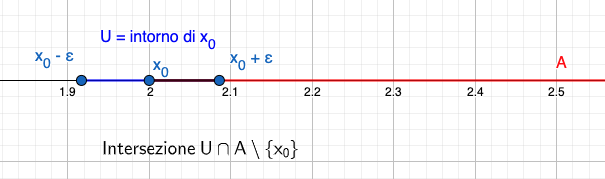
\includegraphics[width=7cm]{images/esempio-intorno-su-estremi.png}
    \caption{Punto di acc $x_0 = 2$ dell'intervallo A}
\end{wrapfigure}

Ora andiamo a dimostrare come tutti i punti [2,3] $\in$ acc(A).
Se poniamo per esempio $x_0 = 2$. Se andiamo a prendere un intorno di $x_0$ nonostante il $\epsilon$ possa essere piccolissimo esisteranno sempre infiniti punti nell'intersezione fra $U$ intorno e $A$ ($U \cap A \setminus \{x_0\}$) perché qualsiasi sia l'epsilon $2 + \epsilon$ rientrerà sempre in A.\\
Questo anche con $x_0 = 3$. 
\begin{note}
Nota che oltre a tutto [2,3] $\in$ A non esisto altri punti di accumulazione di un intervallo A.
\end{note}

\begin{definition}[Punto isolato]
    Dato un insieme A, $x_0 \in A$ si dice \textbf{punto isolato} di A se esiste un $U$ intorno di $x_0$ tale che $U \cap A = \{x_0\}$
\end{definition}
\begin{example}
    Facciamo un osservazione con un intorno spezzato per vedere un caso di punto isolato.
\end{example}
\begin{wrapfigure}{l}{8cm}
    \centering
    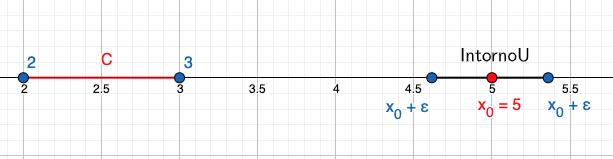
\includegraphics[width=7.3cm, height=2.7cm]{images/esempio-intorno-sepezzato.png}
    \caption{Punto di acc $x_0 = 5$ dell'intervallo C}
\end{wrapfigure}

Se prendiamo un punto C = $(2,3) \cup \{5\}$ non possiamo dire che tutti i punti dell'intervallo C siano punti di accumulazione perché se prendiamo $x_0 = 5$ possono esistere dei casi in cui il suo intorno non interseca C (con U intorno di $x_0 = 5$, $U \cap C \setminus {5} = \O$).\\
Diciamo quindi che in questo caso acc(c) = [2,3]\\\\
\begin{example}
    Esempio in cui verifichiamo come, dato un insieme D = $(3, +\infty)$, sia $+\infty \in$ acc(D).\\
    Come prima cosa prendiamo un $U$ intorno di $x_0 = +\infty$. Quindi $U = (a, +\infty)$.\\
    Definiamo ora il punto maggiore fra 3 ed $a$, $b =$ max($3,a$), questo punto sarà l'estremo sinistro dei punti di accumulazione.
    Facciamo ora l'intersezione:
    \begin{center}
        $U \cap D \setminus \{x_0\} = (2, +\infty) \cap (a, +\infty) \setminus {+\infty} = (b, +\infty) \neq \O$.
    \end{center}
    Vediamo dunque che $+\infty$ è un punto i accumulazione di D, quindi acc(D) = $[b, +\infty]$.
\end{example}
\newpage
\begin{example}
    Esempio prendendo come insieme $E = \mathbb{N}$.
\end{example}
\begin{wrapfigure}{r}{7cm}
    \vspace{-15pt}
    \centering
    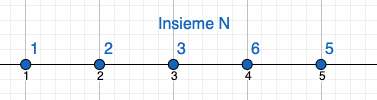
\includegraphics[width=6.2cm]{images/insieme-N.png}
    \caption{Insieme $\mathbb{N}$}
    \label{fig:insieme-N}
\end{wrapfigure}

Se osserviamo l'immagine \ref{fig:insieme-N} vediamo chiaramente come tutti gli elemento di $\mathbb{N}$ sia punti isolare e quindi non siano punti di accumulazione. Ma, per l'esempio visto sopra, $+\infty$ è l'unico punto di accumulazione di $\mathbb{R}$. Acc($\mathbb{N}$) = $+\infty$. \\
\begin{note}
    Allo stesso modo prendendo in considerazione l'insieme $\mathbb{Z}$ i suoi punti di accumulazione sono acc($\mathbb{Z}$) = $\{-\infty, +\infty\}$
\end{note}
\begin{definition}
    Dato un insieme $A \subset \mathbb{R}$, ed un $x_0 \in A$, si dice $x_0$ punto interno ad A se esiste un $U$ intorno di $x_0$ tale che $U \subset A$. L'insieme dei punti interni si indica con int(A).
\end{definition}
\begin{example}
    Dato un A = [3, 5] i punti intesi sono (3,5) e non [3,5] perché se prendiamo $x_0 = 3$ o $x_0 = 5$ essendo che l'intorno di $x_0$ è [$x_0 - \epsilon$, $x_0 + \epsilon$] rimarrà sempre una parte fuori, in particolare quella di sinistra per $x_0 = 3$, e quella di destra per $x_0 = 5$.
\end{example}

\subsubsection{Minimi e massimi locali}
\begin{definition}[Minimi e massimi locali e locali stretti]
    Dato un insieme $A \subset \mathbb{R}$, una funzione $f: A \longrightarrow \mathbb{R}$ ed un punto $x_0 \in A$ si dice che $x_0$ è:
    \begin{itemize}
        \item \textbf{Minimo locale} (o relativo) se esiste un $U$ intorno di $x_0$ tale che $f(x) \geq f(x_0) \: \forall \: x \in U \cap A$
        \item \textbf{Minimo locale stretto} se esiste un $U$ intorno di $x_0$ tale che $f(x) > f(x_0) \: \forall \: x \in U \cap A \setminus \{x_0\}$
        \item \textbf{Massimo locale} (o relativo) se esiste un $U$ intorno di $x_0$ tale che $f(x) \leq f(x_0) \: \forall \: x \in U \cap A$
        \item \textbf{Massimo locale stretto} se esiste un $U$ intorno di $x_0$ tale che $f(x) < f(x_0) \: \forall \: x \in U \cap A \setminus \{x_0\}$
    \end{itemize}
\end{definition}
Questa definizione vuol dire che se andiamo a prendere un intorno di $x_0$, il punto $x_0$ può essere definito minimo o massimo di quel determinato intorno se è il punto più "in basso" o più "in alto" rispetto a tutti gli altri punti dell'intorno.
\begin{figure}[h!]
    \begin{subfigure}{.5\textwidth}
        \centering
        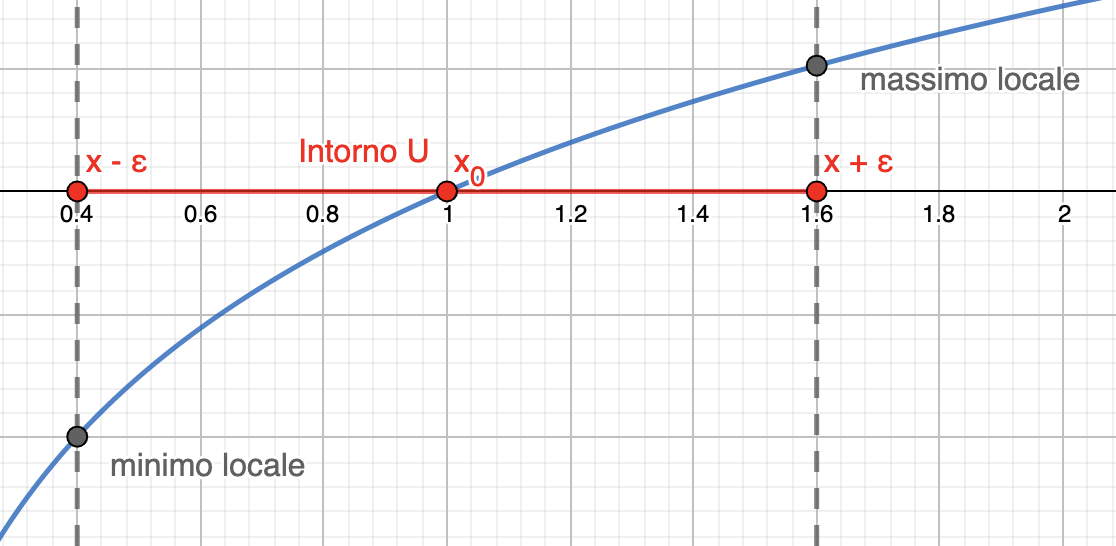
\includegraphics[width=7.7cm]{images/min-max-locale.png}
        \caption{Minimo e massimo locale}
        \label{fig:min-max-locale}
    \end{subfigure}
    \begin{subfigure}{.5\textwidth}
        \centering
        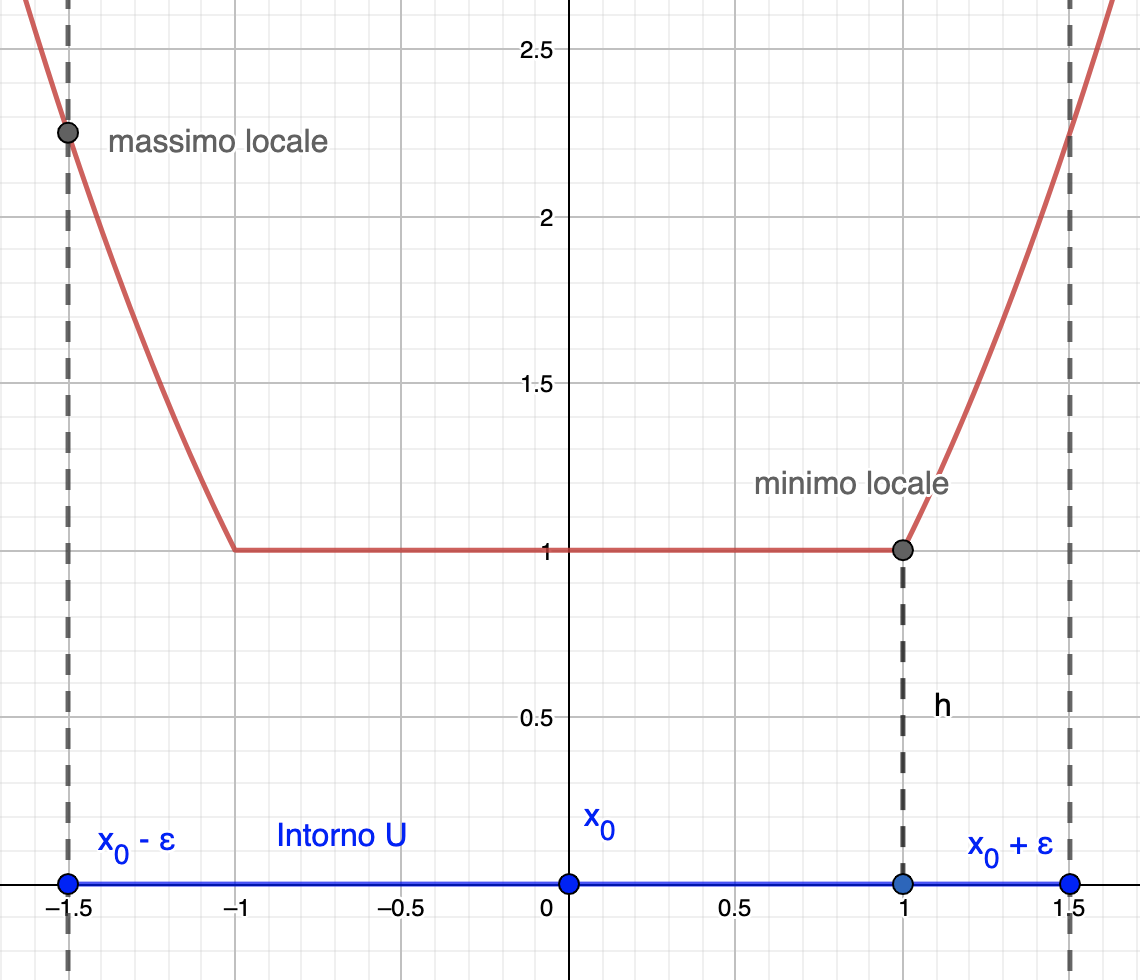
\includegraphics[width=5.5cm]{images/min-max-locale-stretto.png}
        \caption{Minimo e massimo locale stretto}
        \label{fig:min-max-locale-stretto}
    \end{subfigure}
\end{figure}

Come si può vedere dalle immagini [\ref{fig:min-max-locale}] [\ref{fig:min-max-locale-stretto}] noi andiamo a considerare solo i punti all'interno dell'intorno di $x_0$, infatti esisterebbero altri punti esterni a $U$ intorno maggiori o minori, ma non li consideriamo.
\begin{note}
    Nota che se $x_0$ è punto di minimo allora è anche punto di minimo locale, qualsiasi sia l'intorno che prendiamo in considerazione.
\end{note}

\subsection{I limiti}
\begin{definition}[Limite]
    Dato un $A \subset \mathbb{R}$, una $f: A \longrightarrow \mathbb{R}$, ed un $x_0$ punto di accumulazione per A, si dice che $l \in \overline{\mathbb{R}}$ è il limite per $x$ che tende a $x_0$ di $f(x)$ se $\forall$ V intorno di $l$, $\exists \: U$ intorno di $x_0$ t.c. $x \in U \cap A \setminus \{x_0\} \Longrightarrow f(x) \in V$
\end{definition}
Questa definizione dice che un valore $l$ per essere definito come limite di una funzione con $x$ che tende a $x_0$ bisogna che per qualsiasi intorno che andiamo a prendere di $l$ deve esistere una intorno di $x_0$ chiamato U tale che, se una $x$ appartiene ad U allora la $f(x)$ apparterrà all'intorno di $l$. \\
Se ci rifacciamo alle definizioni di intorno vediamo che $x \in U \cap A \setminus \{x_0\}$ vuol dire che $|x-x_0| < \delta$ e che $f(x) \in V $ vuol dire che $l - \epsilon < f(x_0) < l + \epsilon$.\\
Questa definizione può essere scritta in altre parole dicendo che:
\begin{center}
    $\lim\limits_{x\to x_0}f(x) = l$\footnote{La notazione $\lim\limits_{x\to x_0}f(x)$ è quella con cui andiamo a scrivere i limiti e vuol dire limite di $f(x)$ con $x$ che tende a $x_0$ è uguale a $l$ valore del limite} $ \Longleftrightarrow \forall \epsilon > 0 \: \: \exists \delta > 0 $ tale che $x \in A, |x - x_0| < \delta \land x \neq x_0 \Longrightarrow |f(x) - f(x_0)| < \epsilon$
\end{center}
\begin{example}
Alcuni esempi di limiti:
\begin{itemize}
    \item $\lim\limits_{x\to x_0}f(x) = \pm \infty$ \hspace{.5cm} $V = (a, \pm \infty)$ \hspace{.5cm} $f(x) \in V$ se e solo se $f(x) > a$\\
    Il risultato di questo limite è $\pm \infty$ se $\forall a \in \mathbb{R} \: \exists \: \delta > 0$ t.c. $|x-x_0|<\delta, x \in A, x\neq x_0 \Longrightarrow f(x) > a$
    \item $\lim\limits_{x\to \pm \infty}f(x) = l$ \hspace{.5cm} se $l \in \mathbb{R}$ se e solo se $x \to \infty$\\
    Il risultato del limite è un valore appartenete a $\mathbb{R}$ se $\forall \epsilon > a \: \exists a \in \mathbb{R}$ t.c. $x > a \Longrightarrow |f(x) - l| < \epsilon$
    \item $\lim\limits_{x\to \pm \infty}f(x) = \pm \infty$ \:
    se e solo se $\forall a \in \mathbb{R} \exists b \in \mathbb{R}$ t.c. $x > b \Longrightarrow f(x) > a$
\end{itemize}
\end{example}
\begin{theorem}[Unicità dei limiti]
Se esiste un limite di $f$ con $x \to x_0$, questo limite è unico.
\end{theorem}

\subsection{Continuità con i limiti}
Rivediamo le definizioni di limiti (con il limite che sia un numero finito)  e continuità accanto:
\begin{enumerate}
    \item $\lim\limits_{x\to x_0}f(x) = l$ con $x_0 \in A$, $l \in \mathbb{R}$ è vera se e solo se $\forall\epsilon > 0 \: \: \exists \delta >0$ t.c. $x \in A, x \neq x_0$ è $|x - x_0| < \delta \Longrightarrow |f(x) - l| < \epsilon$
    \item $f$ è continua in $x_0$ se e solo se $\forall \epsilon > 0 \: \: \exists \delta > 0$ t.c. $|x - x_0| < \delta$ con $x \in A \Longrightarrow |f(x) - f(x_0)| < \epsilon$
\end{enumerate}
Notiamo subito che fra la definizione (1) e la (2) c'è come unica differenza che nella prima c'è $l$ mentre nella seconda c'è $f(x)$. Possiamo dunque trarre una serie di osservazioni.
\begin{observation}
Data una funzione $f(x)$ essa è continua in $x_0 \Longrightarrow \lim\limits_{x\to x_0}f(x) = l$
\end{observation}
\begin{observation}
Una funzione è sempre continua nei punti isolati.
\end{observation}
\begin{observation}
Nella definizione di limite non serve che $x_0$ sia nel dominio di una funzione, basta che sia un punto di accumulazione per il dominio.
\end{observation}
\begin{example}
Esempio di continuità con i limiti:
\end{example}
\begin{wrapfigure}{r}{6cm}
    \vspace{-50pt}
    \centering
    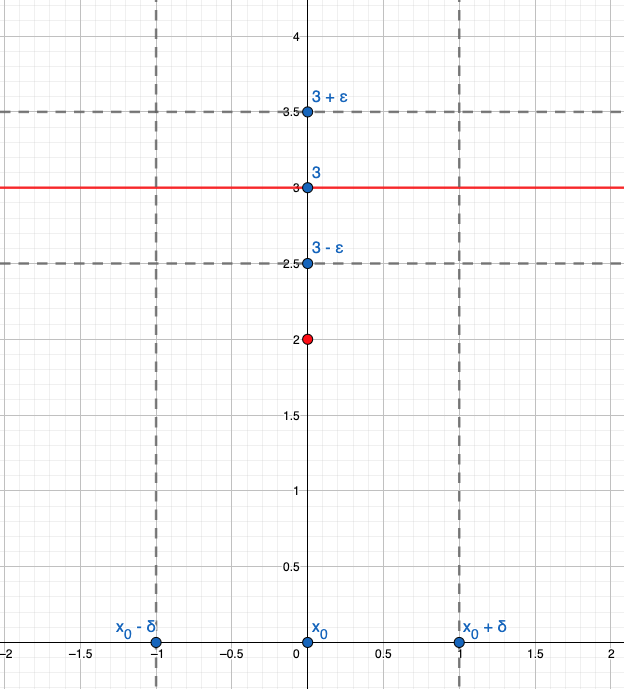
\includegraphics[width=5cm, height=4.7cm]{images/es-continuita-limiti.png}
    \caption{$\lim\limits_{x\to 0}f(x) = 3$}
\end{wrapfigure}

$f(x) = 
    \begin{cases}
        3 \: \: se & x \neq 0 \\
        2 \: \: se & x = 0
    \end{cases}
    $\\ \\
$\lim\limits_{x\to 0}f(x) = 3$, senza considerare f in $x = 0$.\\
Secondo la definizione di continuità di una funzione vista sopra (dove andiamo a guardare il valore del limite in $x_0$):
\begin{center}
    $|x - x_0| < \delta$, $x \in A$, $x \neq x_0$ allora $|f(x) - l| < \epsilon$.
\end{center}
Se andiamo però a vedere $\lim\limits_{x\to 0}f(x) = 3$ mentre $f(0) = 2$ e ovviamente $2 \neq 3$ quindi f non è continua in $x_0$.



\subsection{Limite destro e sinistro}
\begin{definition}[Limite destro e sinistro]
    Se dato un $A \subset \mathbb{R}$, un $x_0 \in Acc(A)$, un $x_0 \in \mathbb{R}$ ($x_0$ deve essere un numero finito), ed  $f: A \to \mathbb{R}$, allora si dice che $l \in \overline{\mathbb{R}}$ è il limite di $f(x)$ per x che tende a $x_0$ da \textbf{destra} (si scrive come $\lim\limits_{x\to x_0^+}f(x) = l$) se:
    \begin{center}
        $\forall \: V$ intorno di $l \: \exists \: \delta > 0$ t.c. $x_0 < x < x_0 + \delta$, $x \in A \Longrightarrow f(x) \in V$
    \end{center}
    Si dice limite \textbf{sinistro} (si scrive come $\lim\limits_{x\to x_0^-}f(x) = l$) se:
    \begin{center}
        $\forall \: V$ intorno di $l \: \exists \: \delta > 0$ t.c. $x_0 - \delta < x < x_0$, $x \in A \Longrightarrow f(x) \in V$
    \end{center}
\end{definition}
\begin{example}
Se prendiamo una $f: (-\infty, 0) \cup (0, +\infty) \to \mathbb{R}$, 
$f(x) = 
    \begin{cases}
        -1 \: \: se & x < 0 \\
        1 \: \: se & x > 0
    \end{cases}
    $ \\ 
    Il $\lim\limits_{x \to 0^+} f(x) = 1$ mentre $\lim\limits_{x \to 0^-} f(x) = -1$. Ciò perché andiamo nel caso del limite destro a guardare il valore "alla destra" di 0 e nel limite sinistro il valore "alla sinistra".
\end{example}
\begin{observation}
$\lim\limits_{x \to x_0^+} = l$ se e solo se $\lim\limits_{x \to x_0^+} = l_1$, $\lim\limits_{x \to x_0^-} = l_2$ e $l_1 = l_2$. Cioè per far in modo che il limite di una funzione che tende ad un valore $x_0$ sia unico bisogna che il limite destre e quello sinistro siano uguali. Nell'esempio precedente infatti possiamo notare che non esiste un unico limite perché i valori del destro e del sinistro sono diversi.
\end{observation}

\subsection{Limite da sopra e da sotto}
Dato un $A \subset \mathbb{R}$, una $f: A \to \mathbb{R}$, ed un $x_0 \in Acc(A)$
\begin{definition}
 Si dice che $\lim\limits_{x \to x_0}f(x) = l^+$ (con $l \in \mathbb{R}$) se $\lim\limits_{x\to x_0}f(x) = l$ ed esiste un $U$ intorno di $x_0$ t.c. $x \in U \cap A \setminus \{x_0\} \Longrightarrow f(x) > l$
\end{definition}
\begin{definition}
 Mentre analogamente si dice che $\lim\limits_{x \to x_0}f(x) = l^-$ (con $l \in \mathbb{R}$) se $\lim\limits_{x\to x_0}f(x) = l$ ed esiste un $U$ intorno di $x_0$ t.c. $x \in U \cap A \setminus \{x_0\} \Longrightarrow f(x) < l$
\end{definition}
Queste due definizione vogliono dire che la funzione può tendere ad un valore "da sopra" nel caso del + e "da sotto" nel caso del -.
\begin{figure}[h!]
    \begin{subfigure}{.5\textwidth}
        \centering
        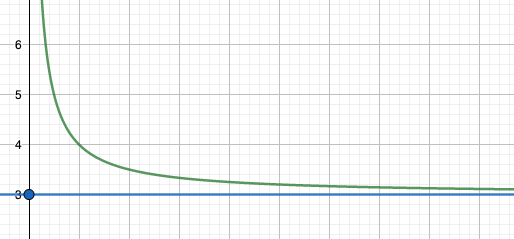
\includegraphics[width=5.5cm]{images/limite-tende-sopra.png}
        \caption{Limite che tende da sopra}
    \end{subfigure}
    \begin{subfigure}{.5\textwidth}
        \centering
        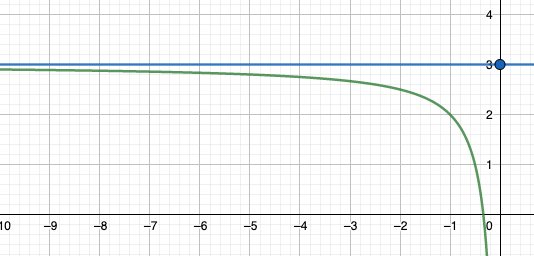
\includegraphics[width=5.5cm]{images/lim-tende-sotto.png}
        \caption{Limite che tende sa sotto}
    \end{subfigure}
\end{figure}
\begin{example}
Un esempio è con $f(x) = \frac{1}{x}$ dove $\lim\limits_{x\to x_0}f(x) = 0^+$
\end{example}

\subsection{Permanenza del segno}
\begin{theorem}[Permanenza del segno]
Dato un $A \subset \mathbb{R}$, un $x_0 \in Acc(A)$ se esiste $\lim\limits_{x\to x_0}f(x) = l$, dove $l \in \overline{\mathbb{R}}$ e $l \neq 0$ allora esiste un intorno $U$ di $x_0$ t.c se $x \in U \cap A \setminus \{x_0\}$ allora $f(x)$ ha lo stesso segno di $l$.
\end{theorem}
\begin{example}
$f: (0, +\infty) \to \mathbb{R}$ \hspace{.5cm} $f(x) = \frac{1}{x}$ \hspace{.5cm} $\lim\limits_{x\to 0^+}f(x) = +\infty$ \\
Quindi visto che $+\infty > 0$ se prendiamo un intorno di $x_0$ qualsiasi $f(x)$ con $x$ appartenente all'intersezione fra il dominio e l'intorno (escluso $x_0$) tornerà che $f(x) > 0$. 
\end{example}

\subsection{Non esistenza di un limite}
Ci sono casistiche di funzioni nel quale un limite non esiste, e quindi no può essere calcolato. Per verificare ciò vediamo alcuni esempi.
\begin{example}
$\lim\limits_{x\to x_0} \sin(x)$ Non esiste. Vediamo perché.
\end{example}
\begin{wrapfigure}{l}{8cm}
    \vspace{-10pt}
    \centering
    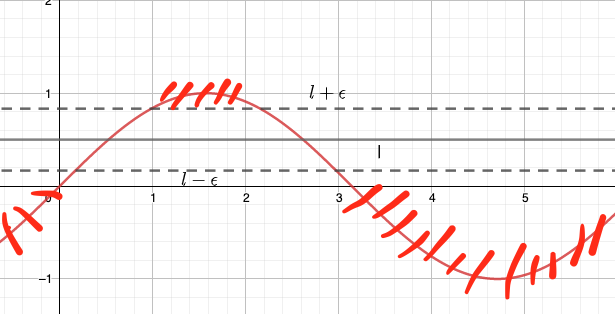
\includegraphics[width=7cm, height=3cm]{images/es-limite-non-esiste.png}
    \caption{Limite che non esiste}
    \label{fig:limite-non-esiste}
\end{wrapfigure}

Supponiamo per assurdo che: \\$\lim\limits_{x\to x_0} \sin(x) = l$\\ \footnote{Ricorda che per la definizione di limite la f(x) deve essere compresa fra $f(x_0) + \epsilon$ e $f(x_0) - \epsilon$ qualsiasi sia il valore di $\epsilon$}Prendiamo ora un valore $\epsilon < \frac{1}{2}$. \\ \\
Se esistesse il limite $l \in \mathbb{R}$ allora dovrebbe esistere $a > 0$ t.c. $x > a \Longrightarrow l - \epsilon < \sin{x} < l + \epsilon$ ma questo assurdo perché vorrebbe dire che $\sin{x}$ oscilla con ampiezza minore di $2\epsilon$ mentre $\sin{x}$ oscilla con ampiezza 2. 
\begin{note}
Nota che nell'immagine \ref{fig:limite-non-esiste} le parti rosse escono dall''intervallo $[l-\epsilon, l+\epsilon]$.
\end{note}

\subsection{Continuità destra e sinistra}
\begin{definition}[Continuità destra e sinistra]\label{continuità-destra-sinistra}
Dato un $A \subset \mathbb{R}$, un $x_0 \in Acc(A)$:
\begin{itemize}
    \item se $\lim\limits_{x \to x_0^+}f(x) = f(x_0)$ allora si dice che $f$ è \textbf{continua a destra} in $x_0$.
    \item se $\lim\limits_{x \to x_0^-}f(x) = f(x_0)$ allora si dice che $f$ è \textbf{continua a sinistra} in $x_0$.
\end{itemize}
\end{definition}

\begin{example}
Data una $
f(x) = \begin{cases}
    1 \: \: se & x \geq 0 \\
    -1 \: \: se & x < 0
\end{cases}$\\
Il $\lim\limits_{0^+}f(x) = 1$ mentre $\lim\limits_{0^-}f(x) = -1$\\
Questo esempio ci dice, come spiegato nella definizione sopra (\ref{continuità-destra-sinistra}), che la funzione è continua a destra nel caso di $0^+$ mentre con $0^-$ la funzione non è continua a sinistra perché il risultato del limite $l \neq f(x_0)$. 
\end{example}
\begin{observation}
    Nel esempio sopra possiamo vedere che la funzione è continua in $x_0^+$ ma non in $x_0^-$. Sin può osservare infatti come una funzione $f$ è continua in un punto $x_0$ se e solo se è continua sia a destra che ha sinistra, perché ciò vorrebbe dire che entrambi i limiti, quello da $x_0^-$ e $x_0^+$, avrebbero uno stesso risultato:
    \begin{center}
        $\lim\limits_{x\to x_0^+}f(x) = l_1$ \:\:\: $\lim\limits_{x\to x_0^-}f(x) = l_2$ \:\:\: $l_1 = l_2 = f(x_0)$
    \end{center}
\end{observation}

\subsection{Teorema di confronto}
\begin{theorem}[Teorema di confronto]
    Dato un $A \subset \mathbb{R}$, un $x_0 \in Acc(x)$, e due funzioni $f,g: A \to \mathbb{R}$. Se esiste un $\lim\limits_{x\to x_0}f(x) = l_1$ e $\lim\limits_{x\to x_0}g(x) = l_2$ e se esiste un $U$ intorno di $x_0$ t.c. $x \in U \cap A \setminus \{x_0\}$ e $f(x) \leq g(x)$ allora $l_1 \leq l_2$.
\end{theorem}
Questo teorema in maniera sintetica dice che se una funzione "sta sotto" l'altra a sua volta anche il limite della prima starà sotto il secondo, detto in altre parole la disuguaglianza passa ai limiti:
\begin{center}
    Se $f(x) \leq g(x)$ allora $\lim\limits_{x\to x_0}f(x) \leq \lim\limits_{x\to x_0}g(x)$
\end{center}

\begin{observation}
    Se però esiste $f(x) < g(x)$ non potrei dire che $\lim\limits_{x\to x_0}f(x) < \lim\limits_{x\to x_0}g(x)$. Perché:
\end{observation}
Se prendiamo come esempio due funzioni una $f(x) = -\frac{1}{x}$ e una $g(x) = \frac{1}{x}$ vediamo che $f(x) < g(x)$ ma se calcoliamo i limiti $\lim\limits_{x\to x_0}f(x) = 0$ e $\lim\limits_{x\to x_0}g(x) = 0$ e quindi i limiti sono uguali. Possiamo dunque dire che le disuguaglianze passano al limite ma diventano sempre deboli:
\begin{center}
        Se $f(x) < g(x)$ allora $\lim\limits_{x\to x_0}f(x) \leq \lim\limits_{x\to x_0}g(x)$
\end{center}

\subsection{Teorema somma e prodotto}
\begin{theorem}[Teorema somma e prodotto]
    Dato un $A \subset \mathbb{R}$, un $x_0 \in Acc(A)$, e due funzioni $f,g: A \to \mathbb{R}$. Supponiamo che esistano i limiti $\lim\limits_{x\to x_0}f(x) = l_1$ e $\lim\limits_{x\to x_0}g(x) = l_2$ con $l_1, l_2 \in \overline{\mathbb{R}}$.
    \begin{itemize}
        \item Se ha senso $l_1 + l_2$ allora esiste $\lim\limits_{x\to x_0}(f + g)(x) = l_1 + l_2$.
        \item Se ha senso $l_1 \cdot l_2$ allora esiste $\lim\limits_{x\to x_0}(f + g)(x) = l_1 \cdot l_2$.
    \end{itemize}
\end{theorem}
\begin{note}
Sono esclusi i casi $l_1 = +\infty$ e $l_2 = -\infty$ (o viceversa) per il prodotto. Sono invece esclusi i casi $l_1 = 0$ e $l_2 = \pm\infty$ (o viceversa) per la somma. Questi casistiche sono dette indeterminate e non possono essere calcolate in maniera diretta.
\end{note}

\subsection{Teorema dei carabinieri}
\begin{theorem}[Teorema dei carabinieri]
    Dato un $A \subset \mathbb{R}$, un $x_0 \in Acc(A)$, e due funzioni $f,g,h: A \to \mathbb{R}$. Se esiste $\lim\limits_{x\to x_0}f(x) = l$ e $\lim\limits_{x\to x_0}h(x) = l$ (i due limiti hanno lo stesso risultato) e se esiste un intorno $U$ di $x_0$ t.c. $x \in A \cup U \setminus \{x_0\}$, se $f(x) \leq g(x) \leq h(x)$ allora esiste $\lim\limits_{x\to x_0}g(x) = l$.
\end{theorem}
Il teorema dei carabinieri dice in maniera sintetica che se due funzioni hanno lo stesso limite ed una è inferiore all'altra se esiste una $g(x)$ in mezzo a queste due funzioni avrà lo stesso limite per uno stesso $x_0$, quindi dall'esistenza dei limiti di $f$ e $h$ (uguali) deduco l'esistenza del limite di $g$
\begin{example}
Facciamo un esempio prendendo $\lim\limits_{x\to +\infty}\frac{2 + \sin{(x)}}{x}$.
Prendendo due funzioni $f(x) = \frac{1}{x}$ e $h(x) = \frac{3}{x}$ sapiamo che $\frac{1}{x} \leq \frac{2 + \sin{(x)}}{x} \leq \frac{3}{x}$. \\
Se poi andiamo a calcolare i limiti per $x \to +\infty$ di $f(x)$ e di $h(x)$ vediamo che $\lim\limits_{x\to +\infty}f(x) = 0$ e $\lim\limits_{x\to +\infty}h(x) = 0$.
Allora per il teorema dei carabinieri $\lim\limits_{x\to +\infty}\frac{2 + \sin{(x)}}{x} = 0$
\end{example}

Alcune conseguenze del teorema dei carabinieri visto sopra:
\begin{proposition}
Dato un $A \subset \mathbb{R}$, un $x_0 \in Acc(A)$, e due funzioni $f,g: A \to \mathbb{R}$:
\begin{itemize}
    \item Se $f$è lim. inferiormente in intorno di $x_0$ e $\lim\limits_{x\to x_0}g(x) = +\infty \Longrightarrow \lim\limits_{x\to x_0}(f + g)(x) = +\infty$.
    \item Se $f$è lim. superiormente in intorno di $x_0$ e $\lim\limits_{x\to x_0}g(x) = -\infty \Longrightarrow \lim\limits_{x\to x_0}(f + g)(x) = -\infty$.
    \item Se $f$è limitata in un intorno di $x_0$ e $\lim\limits_{x\to x_0}g(x) = 0 \Longrightarrow \lim\limits_{x\to x_0}(f \cdot g)(x) = 0$.
\end{itemize}
\end{proposition}

\begin{example}
Prendiamo il $\lim\limits_{x\to +\infty}x + \sin(x)$\\
$\lim\limits_{x\to +\infty}x = +\infty$ \hspace{.5cm} $\lim\limits_{x\to +\infty}\sin(x)$ non esiste.\\
Data l'inesistenza del secondo limite non posso applicare il teorema sul limite della somma ma $\sin(x)$ è limitata inferiormente quindi:
Per il teorema dei carabinieri $x - 1 \leq x + \sin(x) \leq x + 2$, e visto che $\lim\limits_{x\to +\infty}x - 1 = +\infty$ e $\lim\limits_{x\to +\infty}x + 2 = +\infty$ possiamo dire che $\lim\limits_{x\to +\infty}\sin(x) = +\infty$
\end{example}

\subsection{Limitatezza funzione con i limiti}
\begin{theorem}
    Dato un $A \subset \mathbb{R}$, un $x_0 \in Acc(A)$, e $f: A \to \mathbb{R}$. Se esiste $\lim\limits_{x\to x_0}f(x) = l$ e $l \in \mathbb{R}$ (quindi $l$ non è $\pm\infty$) allora $f$ è limitata in un intorno di $x_0$ cioè $\exists \: U$ intorno di $x_0$ e $\exists M \in \mathbb{R}$ con $M > 0$ t.c. $x \in U \cap A \Longrightarrow |f(x)| \leq M$.
\end{theorem}
Questo teorema dice che se prendiamo una funzione che ha un limite per $x\to x_0$ che è un valore diverso da $\pm\infty$ e prendiamo un intorno di $x_0$ esisterà un valore M dove per qualsiasi $x \in U \cap A$ il $|f(x)| \leq M$ che corrisponderebbe a $-M \leq f(x) \leq M$ quindi la funzione sarà limitata nell'intorno selezionato.
\begin{example}
Se prendiamo $f(x) = \frac{1}{x}$ è limitata in un intorno di $+\infty$ perché $\lim\limits_{x\to x_0}f(x) = 0$.
\end{example}

\begin{definition}
Dato un $A \subset \mathbb{R}$, un $x_0 \in Acc(A)$, e $f: A \to \mathbb{R}$ possiamo dire che:
\begin{itemize}
    \item Se $\lim\limits_{x\to x_0}f(x) = 0$ allora si dice che $f$ è \textbf{infinitesima} per $x$ che tende a $x_0$.
    \item Se $\lim\limits_{x\to x_0}f(x) = +\infty$ allora si dice che $f$ è \textbf{diverge positivamente} per $x$ che tende a $x_0$.
    \item Se $\lim\limits_{x\to x_0}f(x) = -\infty$ allora si dice che $f$ è \textbf{diverge negativamente} per $x$ che tende a $x_0$.
    \item Se $\lim\limits_{x\to x_0}f(x) = l$ ed $l \in \mathbb{R}$ ($l$ è finito) allora si dice che $f$ è \textbf{converge} in $l$ per $x$ che tende a $x_0$.
\end{itemize}
\end{definition}

\subsection{Forme indeterminate}
\begin{table}[h!]
    \setlength{\tabcolsep}{7pt}
    \renewcommand{\arraystretch}{1.5}
    \centering
    \begin{tabular}{|c c c|}
        \hline
        $[1]$ $(+\infty) + (-\infty)$ & $[2]$ $(-\infty) + (+\infty)$ & $[3]$ $0 \cdot (\pm \infty)$ \\
        $[4]$ $(\pm \infty)^0$ & $[5]$ $(0^+)^0$ & $[6]$ $(1)^{\pm \infty}$\\ 
        \hline
    \end{tabular}
    \caption{Forme indeterminate}
\end{table}
\begin{demostration}
Dimostriamo come la forma [1] e la [2] siano indeterminate (facciamo un esempio considerandone una, ma sono equivalente).\\
Prendiamo un $f(x) = 2x$ e $g(x) = -x$ e facciamo i limiti di entrambi, ed il limite della somma.\\\\
$\lim\limits_{x\to +\infty}f(x) = +\infty$ e $\lim\limits_{x\to +\infty}g(x) = -\infty$, la somma $\lim\limits_{x\to +\infty}(f + g)(x) = 2x - x = x = +\infty$\\
In questo cosa il limite di $(+\infty) + (-\infty)$ torna $+\infty$.\\ \\
Ora prendiamo invece altre due funzioni $f(x) = \frac{x}{2}$ e $g(x) = -x$ e calcoliamo come prima i limiti di entrambi ed il limite della loro somma.\\\\
$\lim\limits_{x\to +\infty}f(x) = +\infty$ e $\lim\limits_{x\to +\infty}g(x) = -\infty$, la somma $\lim\limits_{x\to +\infty}(f + g)(x) = (\frac{x}{2} - x) = -\frac{x}{2} = -\infty$\\
In questo caso invece il limite di $(+\infty) + (-\infty)$ torna $-\infty$.\\\\
Alla domanda, quale scegliamo? La risposta è nessuna delle due, infatti non potendo avere un risultato fisso diciamo che questa è una forma indeterminata.\\
Nota che questa dimostrazione è valida anche per la forma $0 \cdot (\pm \infty)$.
\end{demostration}
Per le forme [4], [5] e [6] possiamo tramite dei calcoli algebrici spiegarle riconducendoci alle prime 3 forme.\\\\
Possiamo infatti vederle come $f(x)^{g(x)} = e^{\log(f(x)^{g(x)}}) = e^{g(x) \cdot \log(f(x))}$ e quindi possiamo analizzare i casi in cui $\lim\limits_{x\to x_0}g(x) \cdot \lim(f(x))$ è indeterminato:
\begin{enumerate}
    \setcounter{enumi}{3}
    \item Con $g\to 0$ e $f\to +\infty \Longrightarrow \log(f(x)) \to +\infty = 0 \cdot +\infty$ (quindi $(+\infty)^0$ è indeterminata).
    \item Con $g\to 0$ e $f\to +0^+ \Longrightarrow \log(f(x)) \to -\infty = 0 \cdot -\infty$ (quindi $(0^+)^0$ è indeterminata).
    \item Con $g\to \pm\infty$ e $f\to 1 \Longrightarrow \log(f(x)) \to 0 = 0 \cdot \pm\infty$ (quindi $(1)^{\pm\infty}$ è indeterminata).
\end{enumerate}

\subsection{Calcolo dei limiti}
\begin{proposition}
Dato un $A \subset \mathbb{R}$, un $x_0 \in Acc(A)$, e $f: A \to \mathbb{R}$ possiamo vedere che nel calcolare alcuni limiti si verificano delle situazioni ricorrenti:
\begin{itemize}
    \item Se $\lim\limits_{x\to x_0}f(x) = 0^+ \Longrightarrow \lim\limits_{x\to x_0}\frac{1}{f(x)} = +\infty$.
    \item Se $\lim\limits_{x\to x_0}f(x) = 0^- \Longrightarrow \lim\limits_{x\to x_0}\frac{1}{f(x)} = -\infty$.
    \item Se $\lim\limits_{x\to x_0}f(x) = +\infty \Longrightarrow \lim\limits_{x\to x_0}\frac{1}{f(x)} = 0^+$.
    \item Se $\lim\limits_{x\to x_0}f(x) = -\infty \Longrightarrow \lim\limits_{x\to x_0}\frac{1}{f(x)} = 0^-$.
    \item Se $\lim\limits_{x\to x_0}f(x) = l$ con $l \neq 0, \pm\infty \Longrightarrow \lim\limits_{x\to x_0}\frac{1}{f(x)} = \frac{1}{l}$.
\end{itemize}
\end{proposition}
\begin{note}
Nota che se abbiamo $\lim\limits_{x\to x_0}f(x) = 0$ (non $0^+$ o $0^-$) non si conclude nulla su $\lim\limits_{x\to x_0}\frac{1}{f(x)}$
\end{note}

\begin{proposition}
Dati due valori $a,b \in \overline{\mathbb{R}}$, una $f:(a,b) \to \mathbb{R}$ con $f$ debolmente crescente. Allora esistono $\lim\limits_{x\to a^+}f(x) = inf(f(x))$ quando $x \in (a,b)$ e $\lim\limits_{x\to b^-}f(x) = sup(f(x))$ con $x \in (a,b)$. (Analogamente con $f$ debolmente crescente)
\end{proposition}

\begin{example}
$f:(9, -\infty)\to \mathbb{R}$ con $f(x) = -\frac{1}{x}$\\
Se calcoliamo i limiti viene che $\lim\limits_{x\to 0^+}-\frac{1}{x} = +\infty = sup(f)$ \hspace{.1cm} mentre $\lim\limits_{x\to 0^-}-\frac{1}{x} = 0 = inf(f)$
\end{example}

\subsubsection{Limiti fondamentali}
\begin{table}[h!]
    \setlength{\tabcolsep}{7pt}
    \renewcommand{\arraystretch}{1.5}
    \centering
    \begin{tabular}{|c c|c|}
        \hline
        $\lim\limits_{x\to +\infty}x^n = +\infty$ & $\lim\limits_{x\to +\infty}\frac{1}{x^n} = \frac{1}{+\infty} = 0$ & $\lim\limits_{x\to +\infty}a^x = +\infty$ e $\lim\limits_{x\to -\infty}a^x = 0^+$ se $a \geq 1$ \\\hline
        $\lim\limits_{x\to +\infty}e^x = +\infty$ & $\lim\limits_{x\to -\infty}e^x = 0^+$ & $\lim\limits_{x\to +\infty}a^x = 1$ e $\lim\limits_{x\to -\infty}a^x = 1$ se $a = 1$  \\\hline
        $\lim\limits_{x\to 0^+}\log(x) = -\infty$ & $\lim\limits_{x\to +\infty}\log(x) = +\infty$ & $\lim\limits_{x\to +\infty}a^x = 0^+$ e $\lim\limits_{x\to -\infty}a^x = +\infty$ se $0 < a < 1$ \\
        \hline
    \end{tabular}
    \vspace{-5pt}
    \caption{Limiti fondamentali}
\end{table}
Questi limiti scritti sopra sono alcuni dei limiti fondamentali (considera quando c'è $n$ come $n\in \mathbb{N}$)

\subsubsection{Limiti di polinomi}
Se prendiamo una funzione generale così definitiva:
\begin{center}
    $p(x) = a_nx^n + a_{n-1}x^{n-1} + ... + a_1x + a_0$ con $a_0, a_1, ..., a_n \in \mathbb{R}$, $n$ è il grado del polinomio $n \in N$
\end{center}
è possibile trovare una standardizzazione per la risoluzione di $\lim\limits_{x\to +\infty}p(x)$
\begin{example}
Prendiamo in $\lim\limits_{x\to +\infty}3x^2 -7x + 1$.\\
Questa è una forma indeterminata $\lim\limits_{x\to +\infty}3x^2 -7x + 1 = +\infty -\infty + 1$, per risolvere si raccogliere:
\begin{center}
    $\lim\limits_{x\to +\infty}3x^2(1 - \frac{7x}{3x^2} + \frac{1}{3x^2}) = \lim\limits_{x\to +\infty}+\infty \cdot (1 - \frac{7x}{+\infty} + \frac{1}{+\infty}) = \lim\limits_{x\to +\infty}+\infty \cdot (1 - 0 + 0) = +\infty$
\end{center}
\end{example}
\hspace{-15pt}Come regola generale presa la funzione $p(x)$ scritta sopra risolviamo il limite tendente a $\pm\infty$ raccogliendo:
\begin{center}
    \vspace{-10pt}
    $\lim\limits_{x\to \pm\infty}p(x) = \lim\limits_{x\to \pm\infty}a_nx^n (1 + \frac{a_{n-1}}{a_n} \cdot \frac{x^{n-1}}{x^n} + ... + \frac{a_{1}}{a_n} \cdot \frac{x}{x^n} + \frac{a_{0}}{a_n} \cdot \frac{1}{x^n})$
\end{center}
Poi visto che i vari $\frac{x^{n-1}}{x^n}$, $\frac{x}{x^n}$ ecc. si annullano e quindi:
\begin{center}
    $\lim\limits_{x\to \pm\infty} a_nx^4 + a_{n-1}x^{n-1} + ... + a_1x + a_0 = \lim\limits_{x\to \pm\infty}a_nx^n$
\end{center}

\subsubsection{Funzioni razionali}
Se prendiamo una situazione $\frac{p(x)}{q(x)}$ con $p,q$ due polinomi quindi
\begin{center}
    $p(x) = a_nx^n + ... + a_1x + a_0$ \hspace{1cm} $q(x) = b_mx^m + ... + b_1x + b_0$
\end{center}
Possiamo sviluppare il limite seguendo la logica vista nei singoli limiti di polinomi:
\begin{center}
    $\lim\limits_{x\to \pm\infty} = \lim\limits_{x\to \pm\infty} \frac{a_nx^n (1 + \frac{a_{n-1}}{a_n}\cdot\frac{x^{n-1}}{x^n} + ... + \frac{a_0}{a_n}\cdot\frac{1}{x^n})}{b_nx^n (1 + \frac{b_{n-1}}{b_n}\cdot\frac{x^{n-1}}{x^n} + ... + \frac{b_0}{b_n}\cdot\frac{1}{x^n})} = \lim\limits_{x\to \pm\infty}\frac{a_nx^n}{b_mx^n}$
\end{center}

\begin{example}
$\lim\limits_{x\to +\infty}\frac{7x^4 + 5x^2}{-2x^3 + x} = \lim\limits_{x\to +\infty}\frac{7x^4}{-2x^3} = \lim\limits_{x\to +\infty}\frac{7x}{-2} = -\infty$
\end{example}

\subsubsection{Limiti notevoli}
In tabella \ref{tab:limiti-notevoli} alcuni limiti notevoli, cioè limiti che all'apparenza possono sembrare il risultato ma che in realtà tornano un risultato finito.
\begin{table}[h!]
    \centering
    \setlength{\tabcolsep}{10pt}
    \renewcommand{\arraystretch}{2.5}
    \begin{tabular}{|c|c|}
        \hline
        $\lim\limits_{x\to 0}\frac{\sin(x)}{x} = 1$ & $\lim\limits_{x\to 0} \frac{1-\cos(x)}{x^2} = \frac{1}{2}$ \\\hline
        $\lim\limits_{x\to 0}\frac{e^x-1}{x} = 1$ & $\lim\limits_{x\to 0}\frac{\log(1+x)}{x} = 1$\\
        \hline
    \end{tabular}
    \caption{Limiti notevoli}
    \label{tab:limiti-notevoli}
\end{table}
\begin{demostration}
Dimostriamo $\lim\limits_{x\to 0} \frac{1-\cos(x)}{x^2} = \frac{1}{2}$.
\begin{enumerate}
    \item $\lim\limits_{x\to 0} \frac{1-\cos(x)}{x^2} = \frac{1}{2} = \frac{(1-\cos(x)) \cdot (1+\cos(x))}{x^2 \cdot (1+\cos(x))}$ \hspace{.7cm} Moltiplico e divido per $(1+\cos(x))$.
    \item $\lim\limits_{x\to 0} \frac{(1-\cos(x)) \cdot (1+\cos(x))}{x^2 \cdot (1+\cos(x))} = \frac{1-\cos^2(x)}{x^2 \cdot (1 + \cos(x))} = \frac{\sin^2(x)}{x^2 \cdot (1 + \cos(x))}$ \hspace{.7cm} Utilizzo le formule goniometriche.
    \item $\lim\limits_{x\to 0}\frac{\sin^2(x)}{x^2 \cdot (1 + \cos(x))} = \lim\limits_{x\to 0}\frac{\sin(x)}{x} \cdot \frac{\sin(x)}{x} \cdot \frac{1}{1 + \cos(x)}$ \hspace{.7cm} Spezziamo la divisioni in 3 parti.
    \item $\lim\limits_{x\to 0}\frac{\sin(x)}{x} = 1$ \: \: $\lim\limits_{x\to 0}\frac{\sin(x)}{x} = 1$ \: \: $\lim\limits_{x\to 0}\frac{1}{1 + \cos(x)} = \frac{1}{1 + 1}$ \hspace{.7cm} Facciamo il limite dei singoli pezzi.
    \item $\lim\limits_{x\to 0}\frac{1-\cos(x)}{x^2} = 1 \cdot 1 \cdot \frac{1}{2} = \frac{1}{2}$ \hspace{.7cm} Dimostrazione finita. $\blacksquare$
\end{enumerate}
\end{demostration}

\subsubsection{Logaritmi e potenze}
Vediamo una serie di casi di calcolo di limiti con logaritmi e potenze.
\begin{itemize}
    \item $\lim\limits_{x\to +\infty}\frac{\log(x)}{x} = \frac{+\infty}{+\infty}$ forma indeterminata.\\
    Eseguiamo un cambio di variali con $y = \log(x)$ e $x = e^y$. Se $x\to +\infty \Longrightarrow y = \log(x) \to +\infty$\\\\
    Torna che $\lim\limits_{x \to +\infty}\frac{\log(x)}{x} = \lim\limits_{y\to +\infty}\frac{y}{e^y} = 0$
    \item $\lim\limits_{x\to +\infty}\frac{(\log(x))^\beta}{x^\alpha}$ con $\alpha, \beta \in \mathbb{R}$ e $\alpha, \beta > 0$\\
    Possiamo risolvere con un cambio di variabile $y = \log(x)$, $x = e^y$ e se $x \to +\infty \Longrightarrow y\to +\infty$\\\\
    Quindi $\lim\limits_{x\to +\infty}\frac{(\log(x))^\beta}{x^\alpha} = \lim\limits_{y \to +\infty}\frac{y^\beta}{(e^y)^\alpha} = \lim\limits_{y \to +\infty}\frac{y^\beta}{e^{y\cdot\alpha}} = 0$  (l'esponenziale cresce più velocemente).
    \item $\lim\limits_{x\to 0^+}x\log(x) = 0 \cdot (-\infty)$ forma indeterminata.\\
    Facciamo il cambio di variabile $y = \log(x)$, e $x = e^y$ con $x\to 0^+ \Longrightarrow y\to -\infty$.\\\\
    $\lim\limits_{x\to 0^+}x\log(x) = \lim\limits_{y\to -\infty}e^y \cdot y = 0^+ \cdot (-\infty)$ ancora indeterminata.\\
    Possiamo fare un altro cambio di varibile con $z = -y$, e $y = -z$ e se $y \to -\infty \Longrightarrow z \to +\infty$\\\\
    $\lim\limits_{y\to -\infty}e^y \cdot y = \lim\limits_{z\to +\infty}e^{-z} \cdot (-z) = \frac{-z}{e^z} = 0$
    \item $\lim\limits_{x\to 0^+}x^\alpha \cdot \log(x)$ con $\alpha > 0$.\\
    Cambio di variabile con $y = x^\alpha$, e $x = y^{\frac{1}{\alpha}}$ e con $x\to 0^+ \Longrightarrow y\to^+$\\\\
    $\lim\limits_{x\to 0^+}x^\alpha \cdot \log(x) = \lim\limits_{y\to 0^+}y \cdot \log(y^{\frac{1}{\alpha}}) = \lim\limits_{y\to 0^+}\frac{y}{\alpha} \cdot \log(y) = \frac{1}{\alpha}\lim\limits_{y\to 0^+} y \cdot \log(y) = 0$ per l'esempio sopra.
\end{itemize}

\subsection{Limite della composizione di funzioni}
\begin{theorem}[Limite della composizione di funzioni]
    Dati $A,B \subset \mathbb{R}$, una $f: A \to B$, ed una $g: B \to \mathbb{R}$, un punto $x_0 \in Acc(A)$. Se esiste $\lim\limits_{x\to x_0}f(x) = y_0$ e $y_0 \in Acc(B)$ e $\exists \lim\limits_{x\to x_0}g(y) = l \in \overline{\mathbb{R}}$ e se verifichiamo almeno delle seguenti ipotesi:
    \begin{enumerate}
        \item $y_0 \in B$ e g è continua in $y_0$.
        \item Esiste $U$ intorno di $x_0$ t.c. se $x \in U \cap A \setminus \{x_0\} \Longrightarrow f(x) \neq y_0$
    \end{enumerate}
    Allora $\lim\limits_{x\to x_0}(g \circ f)(x) = l$. Cioè:
    \begin{center}
        \vspace{-5pt}
        $\lim\limits_{x\to x_0}(g \circ f)(x) = \lim\limits_{y\to y_0}g(y)$
    \end{center}
\end{theorem}
\begin{example}
Facciamo un esempio andando a calcolare il $\lim\limits_{x\to -\infty}\arctan(x^2)$.\\
Questo limite è una composizione fra $f(x) = x^2$ e $g(y) = \arctan(y)$, che può essere scritto come $(g \circ f)(x) = g(f(x)) = g(x^2) = \arctan(x^2)$.\\
Noi abbiamo che $x_0 = -\infty$ mentre $t_0 = \lim\limits_{x\to x_0}f(x) = \lim\limits_{x\to -\infty}x^2 = +\infty$.\\
Vediamo dunque che l'ipotesi (1) non è verificata perché $y_0 = +\infty$ e non appartiene al dominio di $g$.\\
Mentre possiamo vedere che l'ipotesi (2) è ovviamente verificata perché chiedo che $f(x) \neq y_0$ cioè $f(x) \neq +\infty$ che è ovviamente sempre vero. Possiamo dunque applicare il teorema:\\
$\lim\limits_{y\to y_0}g(y) = \lim\limits_{y\to +\infty}\arctan(y) = \frac{\pi}{2} \Longrightarrow \lim\limits_{x\to -\infty}\arctan(x^2) = \frac{\pi}{2}$
\end{example}
\begin{observation}
    Quello che osserviamo nel teorema del limite della composizione di funzioni + un teorema di cambiamento di variabili. Infatti andando a prendere l'esempio di prima vediamo che:
    \begin{center}
        Da $\lim\limits_{x\to +\infty}\arctan(x^2)$ cambiamo variabile e ponto $y = x^2$, $\lim\limits_{y\to +\infty}\arctan(y) = \frac{\pi}{2}$
    \end{center}
    Nel caso $x\to -\infty$ dobbiamo vedere a quanto tende $y$, quindi $\lim\limits_{x\to -\infty} = \lim\limits_{x\to -\infty}x^2 = +\infty$
\end{observation}
\begin{observation}
    Un altra osservazione è del perché è inserita l'ipotesi (2) nel teorema. Facciamo un esempio per capire il suo scopo.\\
    Prendiamo $f: \mathbb{R} \to \mathbb{R}$, definita come $f(x) = 1 \forall x \in \mathbb{R}$.\\
    Poi prendiamo anche una $g: \mathbb{R} \to \mathbb{R}$ definita come $g(x) = \begin{cases}
        3 se & y = 1\\
        5 se & y \neq 1\\
    \end{cases}$. Facciamo la composizioni di queste due funzioni e valutiamo il limite con $x\to 0$.\\
    $(g \circ f)(x) = g(f(x)) = g(1) = 3 \forall x \in \mathbb{R} \Longrightarrow \lim\limits_{x\to 0}(g \circ f)(x) = 3$.
    Ma  $\lim\limits_{y \to y_0}g(y) = \lim\limits_{y\to 1}g(y) = 5$.\\
    $y_0 = \lim\limits_{x \to x_0}f(x) = \lim\limits_{x\to 0}f(x) = 1$.\\
    Vediamo dunque che $\lim\limits_{x\to x_0} \neq \lim\limits_{y \to y_0}g(y)$.\\
    Ma infatti in questo esempio non abbiamo considerato che non vale l'ipotesi (2) e nemmeno la (1).
\end{observation}

\subsection{Teorema di Weirstrass generalizzato}
\begin{theorem}[Teorema di Weirstrass generalizzato]
Siano $a,b \in \overline{\mathbb{R}}$ e $f: (a,b) \to \mathbb{R}$ continua t.c. $\exists \: \lim\limits_{x \to a}f(x) = l_1$ e $\exists \: \lim\limits_{x \to b}f(x) = l_2$, valgono i seguenti risultati:
\begin{enumerate}
    \item $f$ è limitata inferiormente $\Longleftrightarrow$ $l_1 \neq -\infty$ e $l_2 \neq -\infty$.
    \item $f$ è limitata superiormente $\Longleftrightarrow$ $l_1 \neq +\infty$ e $l_2 \neq +\infty$.
    \item $f$ è limitata  $\Longleftrightarrow$ $l_1 \in \mathbb{R}$ e $l_2 \in \mathbb{R}$.
    \item $f$ ha minimo $\Longleftrightarrow \: \exists x_0 \in (a,b)$ t.c. $f(x_0) \leq min\{l_1, l_2\}$.
    \item $f$ ha massimo $\Longleftrightarrow \: \exists x_0 \in (a,b)$ t.c. $f(x_0) \geq max\{l_1, l_2\}$.
 \end{enumerate}
\end{theorem}
\begin{observation}
I risultati precedenti valgono anche nel caso $a \in \mathbb{R}$ e $f: [a,b) \to \mathbb{R}$ oppure $b\in \mathbb{R}$ e $f: (a,b] \to \mathbb{R}$ (f sempre continua).
\end{observation}
\begin{wrapfigure}[9]{l}{9cm}
    \vspace{-10pt}
    \centering
    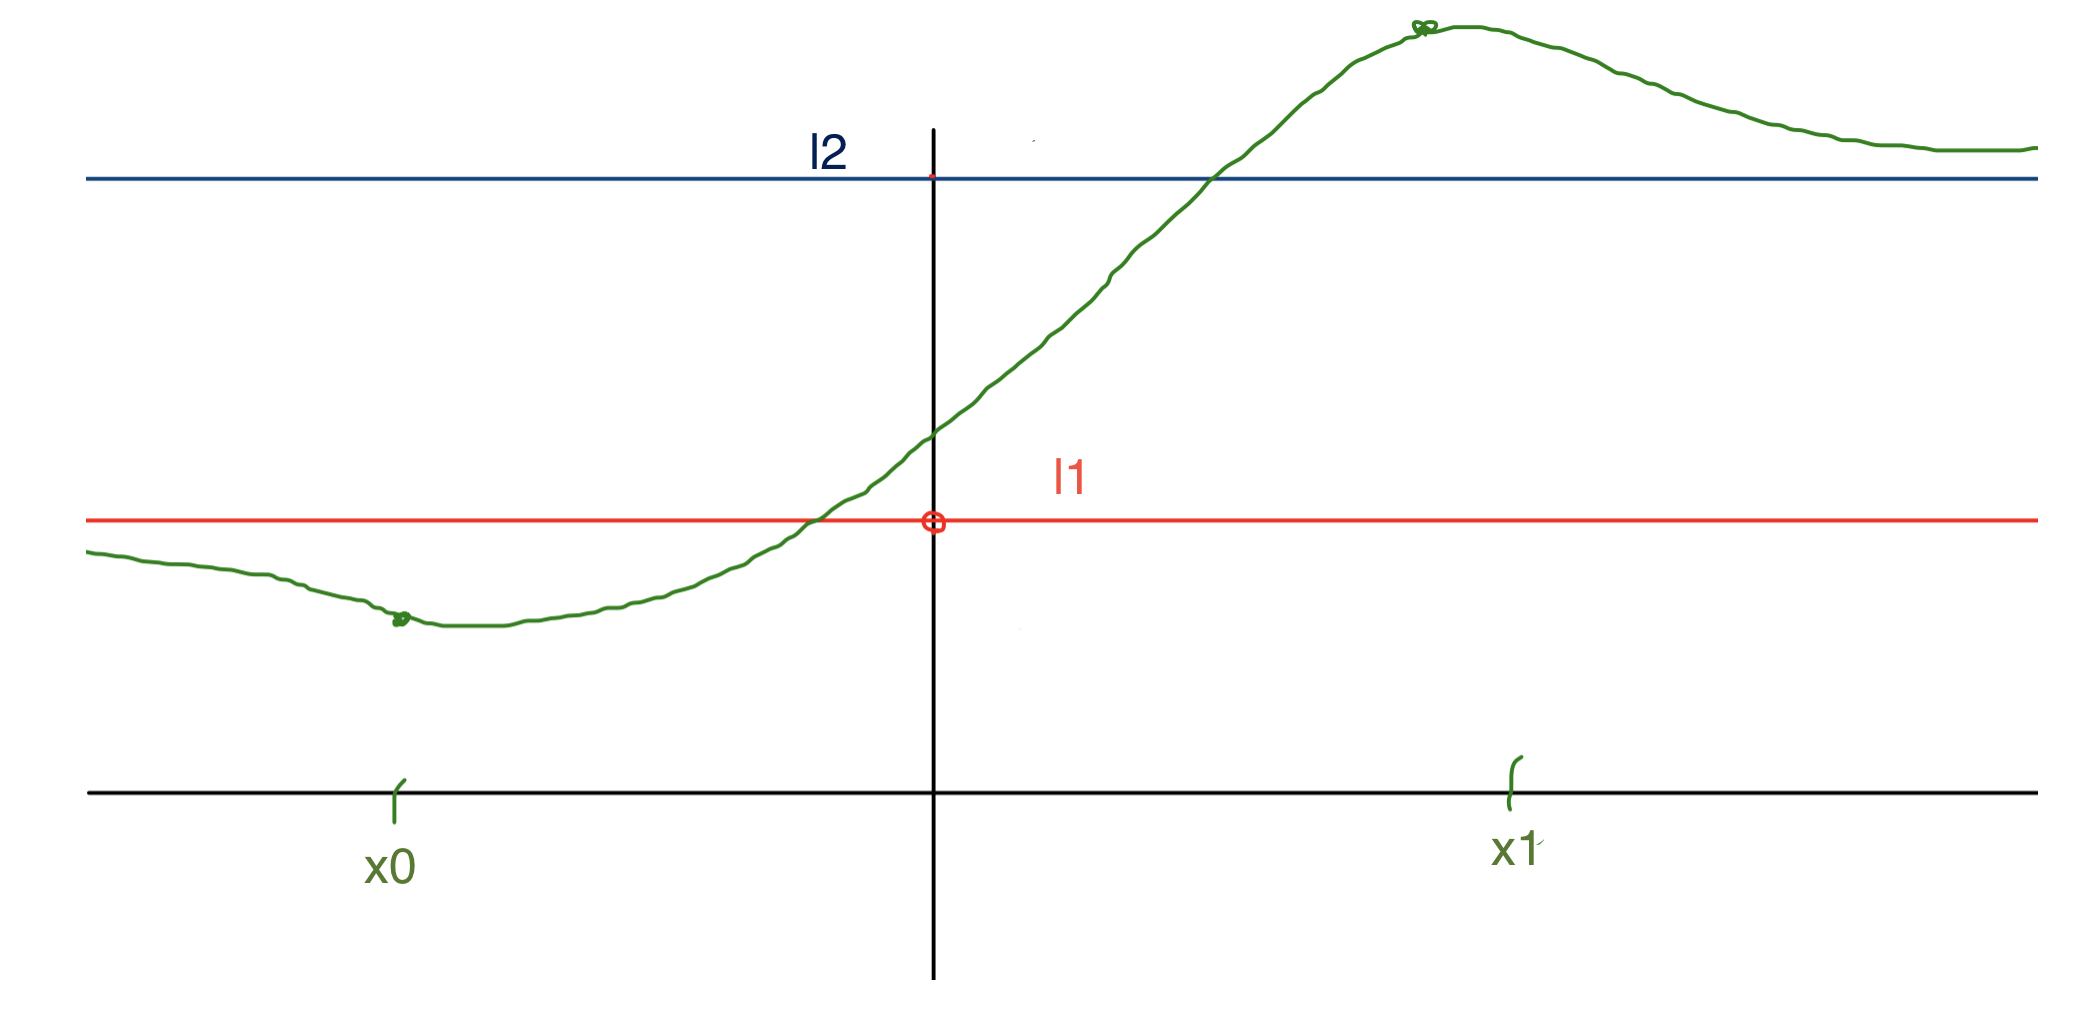
\includegraphics[width=8cm]{images/es-weirstrass-generalizzato.png}
    \vspace{-7pt}
    \caption{Massimi e minimi con Weirstrass}
    \label{fig:werstrass-generalizzato}
\end{wrapfigure}

Come possiamo vedere nella figura \ref{fig:werstrass-generalizzato} se la funzione sale sopra il limite maggiore dovrà necessariamente scendere e quindi si andrà a creare un massimo.\\\\
Ugualmente se la funzione scende sotto il limite minore vuol dire che poi risalirà creando dunque un minimo.\\\\\\

\begin{example}
Prendiamo $f(x) = \frac{1}{x - x^2}$ definita in $f:(0,1) \to \mathbb{R}$ e calcoliamo il limite agli estremi:\\ \\
$\lim\limits_{x\to 0^+}\frac{1}{x \cdot (1 - x)} = \frac{1}{0^+ \cdot 1} = \frac{1}{0^+} = +\infty$ \hspace{.7cm}
$\lim\limits_{x\to 1^-}\frac{1}{x \cdot (1 - x)} = \frac{1}{1 \cdot (1 - 1^-)} = \frac{1}{1 \cdot 0^+)} = \frac{1}{0^+} = +\infty$\\ \\
In questo caso per il teorema visto la funzione $f(x)$ ha minimo.
\end{example}
\begin{example}
Con $f(x) = \frac{x^2 + x|x| + x}{1 + x^2}$ che va da $f: \mathbb{R}\to \mathbb{R}$ verifichiamo se c'è massimo e o minimo.\\
$f(x) = \begin{cases}
    \frac{2x^2 + x}{1 + x^2}& se \: \: x \geq 0\\
    \frac{x}{1 + x^2}& se \: \: x < 0\\
\end{cases}$ \hspace{.7cm} $\lim\limits_{x\to +\infty}\frac{x^2 + x|x| + x}{1 + x^2} = 2 $ \hspace{.3cm} $\lim\limits_{x\to -\infty}\frac{x^2 + x|x| + x}{1 + x^2} = 0 $\\\\
Quello che ci dobbiamo domandare è se $\exists x_0$ t.c. $f(x) \leq 0$ e o $f(x) \geq 2$.\\\\
Se $x<0 \Longrightarrow f(x) = \frac{2x^2 + x}{1 + x^2} < 0 \forall x < 0$ quindi $f$ ha minimo.\\
Mentre se $x \geq 0 \Longrightarrow f(x) = \frac{x}{1 + x^2} \geq 0 \Longrightarrow 2x^2 + x \geq 2 + 2x^2 \Longrightarrow x \geq 2$ quindi $f$ ha anche massimo.
\end{example}